\documentclass[12pt,]{article}
\usepackage[utf8]{inputenc}
\usepackage[T1]{fontenc}
\usepackage{mathptmx}
\usepackage{geometry}
\usepackage{mathtools}
\usepackage[english]{babel}
\usepackage{graphicx}
\usepackage{stackengine}
\usepackage[os=win]{menukeys}
\usepackage{hyperref}
\usepackage{minted}
\usepackage{xcolor}
\usepackage{tikz}
\usepackage[yyyymmdd,hhmmss]{datetime}
\usepackage{etoolbox}
\usepackage{booktabs}

\patchcmd{\thebibliography}{\section*{\refname}}{}{}{}

\newcommand{\ShowOsVersion}{
	\immediate\write18{\unexpanded{foo=`uname -sro` && echo "${foo}" > tmp.tex}}
	\input{tmp}\immediate\write18{rm tmp.tex}
}

\newcommand{\ShowTexVersion}{
	\immediate\write18{\unexpanded{foo=`pdflatex -version | head -n1 | cut -d' ' -f1,2` && echo "${foo}" > tmp.tex}}
	\input{tmp}\immediate\write18{rm tmp.tex}
}

\addto\captionsenglish{\renewcommand{\contentsname}{Daftar Isi}}

\hypersetup{
	colorlinks=true, %set true if you want colored links
	linktoc=all,     %set to all if you want both sections and subsections linked
	linkcolor=blue,  %choose some color if you want links to stand out
	urlcolor=blue,	 %url color
}

\geometry{
	legalpaper,
	left=15mm,
	right=10mm,
	top=10mm,
	bottom=15mm,
}

\title{\Large \bf
	Draft Design Tombol\\
}

\author{Achmadi ST MT}

\date{}

\hypersetup{citecolor=black}

\definecolor{LightGray}{gray}{0.95}

%\pagecolor[rgb]{0.1,0.1,0.1}
%\color[rgb]{1,1,1}

\begin{document}
	\maketitle
	\thispagestyle{empty}
	
	\vspace*{600pt}
	
	\noindent This document written using: \\
	OS : \ShowOsVersion \\
	TeX : \ShowTexVersion \\
	Update: {\today} at \currenttime \\
	
	%%%%%%%%%%%%%%%%%%%%%%%%%%%%%%%%%%%%%%%%%%%%%%%%%%%%%%%%%%%%%%%%%
	
	\newpage
	\begin{figure}[!ht]
		\centering
		\includegraphics[width=500pt]{iface}
		\caption{Tombol Pengguna}
	\end{figure}

	%%%%%%%%%%%%%%%%%%%%%%%%%%%%%%%%%%%%%%%%%%%%%%%%%%%%%%%%%%%%%%%%%
	
	\newpage
	\section{Daftar Tombol}
	
	Berikut Daftar Tombol untuk Pengguna (diluar Tombol Audiometri):
	
	\begin{table}[H]
		\begin{tabular}{|c|c|}
			\toprule
			
			\raisebox{-\totalheight}{
\includegraphics[width=0.05\textwidth]{symbols/power}} & SMD Slide Switch untuk power\textbf{*}
			\\ \midrule
			
			\raisebox{-\totalheight}{
\includegraphics[width=0.05\textwidth]{symbols/file_last}} & Seleksi file rekaman langsung memilih rekaman terakhir
			\\ \midrule
			
			\raisebox{-\totalheight}{
\includegraphics[width=0.05\textwidth]{symbols/file_scroll}} & Seleksi file rekaman secara berurutan berulang
			\\ \midrule
			
			\raisebox{-\totalheight}{
\includegraphics[width=0.05\textwidth]{symbols/page}} & Berpindah halaman yang ditampilkan LCD\textbf{**}
			\\ \midrule
			
			\raisebox{-\totalheight}{
\includegraphics[width=0.05\textwidth]{symbols/wifi}} & Berpindah mode ESP dari Access-Point ke Station atau sebaliknya
			\\ \midrule
			
			\raisebox{-\totalheight}{
\includegraphics[width=0.05\textwidth]{symbols/upload}} & POST request JSON data rekaman ke server
			\\ \midrule
		\end{tabular}
	\end{table}

	\textbf{*}) Contoh SMD Power Switch Slide yang dipilih:
	
	\begin{figure}[!ht]
		\centering
		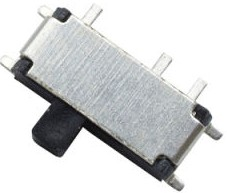
\includegraphics[width=100pt]{symbols/msk12c02}
		\caption{MSK12C02}
	\end{figure}

	\textbf{**}) Rencana halaman yang akan ditampilkan di LCD:
	\begin{itemize}
		\item \textbf{Home}. Sebagai halaman pertama yang muncul setelah power on.
		Menampilkan informasi antara lain:
		\begin{itemize}
			\item Persen Battery
			\item Mode ESP sedang dalam Station atau Access Point
			\item Informasi Koneksi seperti IP dan SSID
			\item Mode Audiometri sedang Idle atau Session\\
			Notes: Saat mode Session, maka tampilan dikunci pada halaman Home
		\end{itemize}
		Dapat diakses dengan tombol Pindah Halaman.
	
		\item \textbf{Daftar File}. Menampilkan daftar file untuk dipilih secara berurutan berulang.\\
		Hanya dapat diakses melalu tombol Seleksi File.
		
		\item \textbf{Upload}. Menampilkan proses kirim data file rekaman terpilih.\\
		Hanya dapat diakses melalu tombol Upload.
		
		\item \textbf{Audiogram}. Menampilkan preview data Audiogram dari file rekaman terpilih.\\
		Dapat diakses dengan tombol Pindah Halaman.
		
		\item \textbf{Metadata}. Menampilkan metadata dari file rekaman terpilih.\\
		Dapat diakses dengan tombol Pindah Halaman.
	\end{itemize}

	\textbf{Tambahan:}
	\begin{itemize}
		\item Untuk tombol memulai Audiometri dan 3-Force Choice tetap menggunakan 3 tombol Audiometri \textbf{A-B-C}.
		\item Port USB untuk komunikasi serial dengan PC tetap diperlukan untuk proses debugging/kontrol selama proses development.
	\end{itemize}

\end{document}